\section{Variable Bias Voltage SRFs}
%==================================
\label{app:Vset}
This appendix contains the comparisons of the low spectral resolution digitized SRFs at low, nominal, and high bias voltages for nominal baseplate temperature (20\textdegree{}C) from the ATMS PFM Calibration Data Book\cite{ATMS_PFM_CalLog}. The digitizations were performed by Lynn Chidester of the Space Dynamics Laboratory (SDL) at Utah State University. Included in the SRF plots are the ``boxcar'' SRF, based on the table \ref{tab:atms_fo_sb_and_df} data, and a representative brightness temperature spectrum.

Shown alongside each SRF comparison are the brightness temperature differences for the SRFs with respect to the boxcar reference response. MonoRTM \cite{Clough_2005} was used to compute the top-of-atmosphere brightness temperatures for the ECMWF83 profile data set \cite{ECMWF_profile_set2,Matricardi_ECMWF564} at the frequencies of the SRFs. These monochromatic brightness temperatures were then integrated over frequency to provide the channel brightness temperatures.

\newpage

\subsection{Channel 1}
\begin{figure}[H]
  \label{fig:Vset.ch1_response}
  \centering
  \begin{tabular}{c}
    \hspace{1.75cm}\sffamily\textbf{Linear y-axis} \\
    \includegraphics[scale=0.55]{graphics/srf/Vset/lin/atms_npp-1.eps} \\
    \hspace{1.75cm}\sffamily\textbf{Base-10 logarithmic y-axis} \\
    \includegraphics[scale=0.55]{graphics/srf/Vset/log/atms_npp-1.eps}
  \end{tabular}
  \caption{ATMS channel 1 response at nominal temperature (20\textdegree{}C) for the three test voltages: $V_{NOM}$, $V_{LO}$, and $V_{HI}$. Vertical dashed lines are the locations of the computed central frequencies. \textbf{(Top)} Linear y-axis. \textbf{(Bottom)} Base-10 logarithmic y-axis.}
\end{figure}

\subsection{Channel 2}
\begin{figure}[H]
  \label{fig:Vset.ch2_response}
  \centering
  \begin{tabular}{c}
    \hspace{1.75cm}\sffamily\textbf{Linear y-axis} \\
    \includegraphics[scale=0.55]{graphics/srf/Vset/lin/atms_npp-2.eps} \\
    \hspace{1.75cm}\sffamily\textbf{Base-10 logarithmic y-axis} \\
    \includegraphics[scale=0.55]{graphics/srf/Vset/log/atms_npp-2.eps}
  \end{tabular}
  \caption{ATMS channel 2 response at nominal temperature (20\textdegree{}C) for the three test voltages: $V_{NOM}$, $V_{LO}$, and $V_{HI}$. Vertical dashed lines are the locations of the computed central frequencies. \textbf{(Top)} Linear y-axis. \textbf{(Bottom)} Base-10 logarithmic y-axis.}
\end{figure}

\subsection{Channel 3}
\begin{figure}[H]
  \label{fig:Vset.ch3_response}
  \centering
  \begin{tabular}{c}
    \hspace{1.75cm}\sffamily\textbf{Linear y-axis} \\
    \includegraphics[scale=0.55]{graphics/srf/Vset/lin/atms_npp-3.eps} \\
    \hspace{1.75cm}\sffamily\textbf{Base-10 logarithmic y-axis} \\
    \includegraphics[scale=0.55]{graphics/srf/Vset/log/atms_npp-3.eps}
  \end{tabular}
  \caption{ATMS channel 3 response at nominal temperature (20\textdegree{}C) for the three test voltages: $V_{NOM}$, $V_{LO}$, and $V_{HI}$. Vertical dashed lines are the locations of the computed central frequencies. \textbf{(Top)} Linear y-axis. \textbf{(Bottom)} Base-10 logarithmic y-axis.}
\end{figure}

\subsection{Channel 4}
\begin{figure}[H]
  \label{fig:Vset.ch4_response}
  \centering
  \begin{tabular}{c}
    \hspace{1.75cm}\sffamily\textbf{Linear y-axis} \\
    \includegraphics[scale=0.55]{graphics/srf/Vset/lin/atms_npp-4.eps} \\
    \hspace{1.75cm}\sffamily\textbf{Base-10 logarithmic y-axis} \\
    \includegraphics[scale=0.55]{graphics/srf/Vset/log/atms_npp-4.eps}
  \end{tabular}
  \caption{ATMS channel 4 response at nominal temperature (20\textdegree{}C) for the three test voltages: $V_{NOM}$, $V_{LO}$, and $V_{HI}$. Vertical dashed lines are the locations of the computed central frequencies. \textbf{(Top)} Linear y-axis. \textbf{(Bottom)} Base-10 logarithmic y-axis.}
\end{figure}

\subsection{Channel 5}
\begin{figure}[H]
  \label{fig:Vset.ch5_response}
  \centering
  \begin{tabular}{c}
    \hspace{1.75cm}\sffamily\textbf{Linear y-axis} \\
    \includegraphics[scale=0.55]{graphics/srf/Vset/lin/atms_npp-5.eps} \\
    \hspace{1.75cm}\sffamily\textbf{Base-10 logarithmic y-axis} \\
    \includegraphics[scale=0.55]{graphics/srf/Vset/log/atms_npp-5.eps}
  \end{tabular}
  \caption{ATMS channel 5 response at nominal temperature (20\textdegree{}C) for the three test voltages: $V_{NOM}$, $V_{LO}$, and $V_{HI}$. Vertical dashed lines are the locations of the computed central frequencies. \textbf{(Top)} Linear y-axis. \textbf{(Bottom)} Base-10 logarithmic y-axis.}
\end{figure}

\subsection{Channel 6}
\begin{figure}[H]
  \label{fig:Vset.ch6_response}
  \centering
  \begin{tabular}{c}
    \hspace{0.75cm}\sffamily\textbf{Linear y-axis} \\
    \includegraphics[scale=0.55]{graphics/srf/Vset/lin/atms_npp-6.eps} \\
    \hspace{0.75cm}\sffamily\textbf{Base-10 logarithmic y-axis} \\
    \includegraphics[scale=0.55]{graphics/srf/Vset/log/atms_npp-6.eps}
  \end{tabular}
  \caption{ATMS channel 6 response at nominal temperature (20\textdegree{}C) for the three test voltages: $V_{NOM}$, $V_{LO}$, and $V_{HI}$. Vertical dashed lines are the locations of the computed central frequencies. \textbf{(Top)} Linear y-axis. \textbf{(Bottom)} Base-10 logarithmic y-axis.}
\end{figure}

\subsection{Channel 7}
\begin{figure}[H]
  \label{fig:Vset.ch7_response}
  \centering
  \begin{tabular}{c}
    \hspace{1.75cm}\sffamily\textbf{Linear y-axis} \\
    \includegraphics[scale=0.55]{graphics/srf/Vset/lin/atms_npp-7.eps} \\
    \hspace{1.75cm}\sffamily\textbf{Base-10 logarithmic y-axis} \\
    \includegraphics[scale=0.55]{graphics/srf/Vset/log/atms_npp-7.eps}
  \end{tabular}
  \caption{ATMS channel 7 response at nominal temperature (20\textdegree{}C) for the three test voltages: $V_{NOM}$, $V_{LO}$, and $V_{HI}$. Vertical dashed lines are the locations of the computed central frequencies. \textbf{(Top)} Linear y-axis. \textbf{(Bottom)} Base-10 logarithmic y-axis.}
\end{figure}

\subsection{Channel 8}
\begin{figure}[H]
  \label{fig:Vset.ch8_response}
  \centering
  \begin{tabular}{c}
    \hspace{1.75cm}\sffamily\textbf{Linear y-axis} \\
    \includegraphics[scale=0.55]{graphics/srf/Vset/lin/atms_npp-8.eps} \\
    \hspace{1.75cm}\sffamily\textbf{Base-10 logarithmic y-axis} \\
    \includegraphics[scale=0.55]{graphics/srf/Vset/log/atms_npp-8.eps}
  \end{tabular}
  \caption{ATMS channel 8 response at nominal temperature (20\textdegree{}C) for the three test voltages: $V_{NOM}$, $V_{LO}$, and $V_{HI}$. Vertical dashed lines are the locations of the computed central frequencies. \textbf{(Top)} Linear y-axis. \textbf{(Bottom)} Base-10 logarithmic y-axis.}
\end{figure}

\subsection{Channel 9}
\begin{figure}[H]
  \label{fig:Vset.ch9_response}
  \centering
  \begin{tabular}{c}
    \hspace{1.75cm}\sffamily\textbf{Linear y-axis} \\
    \includegraphics[scale=0.55]{graphics/srf/Vset/lin/atms_npp-9.eps} \\
    \hspace{1.75cm}\sffamily\textbf{Base-10 logarithmic y-axis} \\
    \includegraphics[scale=0.55]{graphics/srf/Vset/log/atms_npp-9.eps}
  \end{tabular}
  \caption{ATMS channel 9 response at nominal temperature (20\textdegree{}C) for the three test voltages: $V_{NOM}$, $V_{LO}$, and $V_{HI}$. Vertical dashed lines are the locations of the computed central frequencies. \textbf{(Top)} Linear y-axis. \textbf{(Bottom)} Base-10 logarithmic y-axis.}
\end{figure}

\subsection{Channel 10}
\begin{figure}[H]
  \label{fig:Vset.ch10_response}
  \centering
  \begin{tabular}{c}
    \hspace{0.75cm}\sffamily\textbf{Linear y-axis} \\
    \includegraphics[scale=0.55]{graphics/srf/Vset/lin/atms_npp-10.eps} \\
    \hspace{0.75cm}\sffamily\textbf{Base-10 logarithmic y-axis} \\
    \includegraphics[scale=0.55]{graphics/srf/Vset/log/atms_npp-10.eps}
  \end{tabular}
  \caption{ATMS channel 10 response at nominal temperature (20\textdegree{}C) for the three test voltages: $V_{NOM}$, $V_{LO}$, and $V_{HI}$. Vertical dashed lines are the locations of the computed central frequencies. \textbf{(Top)} Linear y-axis. \textbf{(Bottom)} Base-10 logarithmic y-axis.}
\end{figure}

\subsection{Channel 11}
\begin{figure}[H]
  \label{fig:Vset.ch11_response}
  \centering
  \begin{tabular}{c}
    \hspace{0.75cm}\sffamily\textbf{Linear y-axis} \\
    \includegraphics[scale=0.55]{graphics/srf/Vset/lin/atms_npp-11.eps} \\
    \hspace{0.75cm}\sffamily\textbf{Base-10 logarithmic y-axis} \\
    \includegraphics[scale=0.55]{graphics/srf/Vset/log/atms_npp-11.eps}
  \end{tabular}
  \caption{ATMS channel 11 response at nominal temperature (20\textdegree{}C) for the three test voltages: $V_{NOM}$, $V_{LO}$, and $V_{HI}$. Vertical dashed lines are the locations of the computed central frequencies. \textbf{(Top)} Linear y-axis. \textbf{(Bottom)} Base-10 logarithmic y-axis.}
\end{figure}

\subsection{Channel 12}
\begin{figure}[H]
  \label{fig:Vset.ch12_response}
  \centering
  \begin{tabular}{c}
    \hspace{0.75cm}\sffamily\textbf{Linear y-axis} \\
    \includegraphics[scale=0.55]{graphics/srf/Vset/lin/atms_npp-12.eps} \\
    \hspace{0.75cm}\sffamily\textbf{Base-10 logarithmic y-axis} \\
    \includegraphics[scale=0.55]{graphics/srf/Vset/log/atms_npp-12.eps}
  \end{tabular}
  \caption{ATMS channel 12 response at nominal temperature (20\textdegree{}C) for the three test voltages: $V_{NOM}$, $V_{LO}$, and $V_{HI}$. Vertical dashed lines are the locations of the computed central frequencies. \textbf{(Top)} Linear y-axis. \textbf{(Bottom)} Base-10 logarithmic y-axis.}
\end{figure}

\subsection{Channel 13}
\begin{figure}[H]
  \label{fig:Vset.ch13_response}
  \centering
  \begin{tabular}{c}
    \hspace{0.75cm}\sffamily\textbf{Linear y-axis} \\
    \includegraphics[scale=0.55]{graphics/srf/Vset/lin/atms_npp-13.eps} \\
    \hspace{0.75cm}\sffamily\textbf{Base-10 logarithmic y-axis} \\
    \includegraphics[scale=0.55]{graphics/srf/Vset/log/atms_npp-13.eps}
  \end{tabular}
  \caption{ATMS channel 13 response at nominal temperature (20\textdegree{}C) for the three test voltages: $V_{NOM}$, $V_{LO}$, and $V_{HI}$. Vertical dashed lines are the locations of the computed central frequencies. \textbf{(Top)} Linear y-axis. \textbf{(Bottom)} Base-10 logarithmic y-axis.}
\end{figure}

\subsection{Channel 14}
\begin{figure}[H]
  \label{fig:Vset.ch14_response}
  \centering
  \begin{tabular}{c}
    \hspace{0.75cm}\sffamily\textbf{Linear y-axis} \\
    \includegraphics[scale=0.55]{graphics/srf/Vset/lin/atms_npp-14.eps} \\
    \hspace{0.75cm}\sffamily\textbf{Base-10 logarithmic y-axis} \\
    \includegraphics[scale=0.55]{graphics/srf/Vset/log/atms_npp-14.eps}
  \end{tabular}
  \caption{ATMS channel 14 response at nominal temperature (20\textdegree{}C) for the three test voltages: $V_{NOM}$, $V_{LO}$, and $V_{HI}$. Vertical dashed lines are the locations of the computed central frequencies. \textbf{(Top)} Linear y-axis. \textbf{(Bottom)} Base-10 logarithmic y-axis.}
\end{figure}

\subsection{Channel 15}
\begin{figure}[H]
  \label{fig:Vset.ch15_response}
  \centering
  \begin{tabular}{c}
    \hspace{0.75cm}\sffamily\textbf{Linear y-axis} \\
    \includegraphics[scale=0.55]{graphics/srf/Vset/lin/atms_npp-15.eps} \\
    \hspace{0.75cm}\sffamily\textbf{Base-10 logarithmic y-axis} \\
    \includegraphics[scale=0.55]{graphics/srf/Vset/log/atms_npp-15.eps}
  \end{tabular}
  \caption{ATMS channel 15 response at nominal temperature (20\textdegree{}C) for the three test voltages: $V_{NOM}$, $V_{LO}$, and $V_{HI}$. Vertical dashed lines are the locations of the computed central frequencies. \textbf{(Top)} Linear y-axis. \textbf{(Bottom)} Base-10 logarithmic y-axis.}
\end{figure}

\subsection{Channel 16}
\begin{figure}[H]
  \label{fig:Vset.ch16_response}
  \centering
  \begin{tabular}{c}
    \hspace{1.75cm}\sffamily\textbf{Linear y-axis} \\
    \includegraphics[scale=0.55]{graphics/srf/Vset/lin/atms_npp-16.eps} \\
    \hspace{1.75cm}\sffamily\textbf{Base-10 logarithmic y-axis} \\
    \includegraphics[scale=0.55]{graphics/srf/Vset/log/atms_npp-16.eps}
  \end{tabular}
  \caption{ATMS channel 16 response at nominal temperature (20\textdegree{}C) for the three test voltages: $V_{NOM}$, $V_{LO}$, and $V_{HI}$. Vertical dashed lines are the locations of the computed central frequencies. \textbf{(Top)} Linear y-axis. \textbf{(Bottom)} Base-10 logarithmic y-axis.}
\end{figure}

\subsection{Channel 17}
\begin{figure}[H]
  \label{fig:Vset.ch17_response}
  \centering
  \begin{tabular}{c}
    \hspace{0.75cm}\sffamily\textbf{Linear y-axis} \\
    \includegraphics[scale=0.55]{graphics/srf/Vset/lin/atms_npp-17.eps} \\
    \hspace{0.75cm}\sffamily\textbf{Base-10 logarithmic y-axis} \\
    \includegraphics[scale=0.55]{graphics/srf/Vset/log/atms_npp-17.eps}
  \end{tabular}
  \caption{ATMS channel 17 response at nominal temperature (20\textdegree{}C) for the three test voltages: $V_{NOM}$, $V_{LO}$, and $V_{HI}$. Vertical dashed lines are the locations of the computed central frequencies. \textbf{(Top)} Linear y-axis. \textbf{(Bottom)} Base-10 logarithmic y-axis.}
\end{figure}

\subsection{Channel 18}
\begin{figure}[H]
  \label{fig:Vset.ch18_response}
  \centering
  \begin{tabular}{c}
    \hspace{0.75cm}\sffamily\textbf{Linear y-axis} \\
    \includegraphics[scale=0.55]{graphics/srf/Vset/lin/atms_npp-18.eps} \\
    \hspace{0.75cm}\sffamily\textbf{Base-10 logarithmic y-axis} \\
    \includegraphics[scale=0.55]{graphics/srf/Vset/log/atms_npp-18.eps}
  \end{tabular}
  \caption{ATMS channel 18 response at nominal temperature (20\textdegree{}C) for the three test voltages: $V_{NOM}$, $V_{LO}$, and $V_{HI}$. Vertical dashed lines are the locations of the computed central frequencies. \textbf{(Top)} Linear y-axis. \textbf{(Bottom)} Base-10 logarithmic y-axis.}
\end{figure}

\subsection{Channel 19}
\begin{figure}[H]
  \label{fig:Vset.ch19_response}
  \centering
  \begin{tabular}{c}
    \hspace{0.75cm}\sffamily\textbf{Linear y-axis} \\
    \includegraphics[scale=0.55]{graphics/srf/Vset/lin/atms_npp-19.eps} \\
    \hspace{0.75cm}\sffamily\textbf{Base-10 logarithmic y-axis} \\
    \includegraphics[scale=0.55]{graphics/srf/Vset/log/atms_npp-19.eps}
  \end{tabular}
  \caption{ATMS channel 19 response at nominal temperature (20\textdegree{}C) for the three test voltages: $V_{NOM}$, $V_{LO}$, and $V_{HI}$. Vertical dashed lines are the locations of the computed central frequencies. \textbf{(Top)} Linear y-axis. \textbf{(Bottom)} Base-10 logarithmic y-axis.}
\end{figure}

\subsection{Channel 20}
\begin{figure}[H]
  \label{fig:Vset.ch20_response}
  \centering
  \begin{tabular}{c}
    \hspace{0.75cm}\sffamily\textbf{Linear y-axis} \\
    \includegraphics[scale=0.55]{graphics/srf/Vset/lin/atms_npp-20.eps} \\
    \hspace{0.75cm}\sffamily\textbf{Base-10 logarithmic y-axis} \\
    \includegraphics[scale=0.55]{graphics/srf/Vset/log/atms_npp-20.eps}
  \end{tabular}
  \caption{ATMS channel 20 response at nominal temperature (20\textdegree{}C) for the three test voltages: $V_{NOM}$, $V_{LO}$, and $V_{HI}$. Vertical dashed lines are the locations of the computed central frequencies. \textbf{(Top)} Linear y-axis. \textbf{(Bottom)} Base-10 logarithmic y-axis.}
\end{figure}

\subsection{Channel 21}
\begin{figure}[H]
  \label{fig:Vset.ch21_response}
  \centering
  \begin{tabular}{c}
    \hspace{0.75cm}\sffamily\textbf{Linear y-axis} \\
    \includegraphics[scale=0.55]{graphics/srf/Vset/lin/atms_npp-21.eps} \\
    \hspace{0.75cm}\sffamily\textbf{Base-10 logarithmic y-axis} \\
    \includegraphics[scale=0.55]{graphics/srf/Vset/log/atms_npp-21.eps}
  \end{tabular}
  \caption{ATMS channel 21 response at nominal temperature (20\textdegree{}C) for the three test voltages: $V_{NOM}$, $V_{LO}$, and $V_{HI}$. Vertical dashed lines are the locations of the computed central frequencies. \textbf{(Top)} Linear y-axis. \textbf{(Bottom)} Base-10 logarithmic y-axis.}
\end{figure}

\subsection{Channel 22}
\begin{figure}[H]
  \label{fig:Vset.ch22_response}
  \centering
  \begin{tabular}{c}
    \hspace{0.75cm}\sffamily\textbf{Linear y-axis} \\
    \includegraphics[scale=0.55]{graphics/srf/Vset/lin/atms_npp-22.eps} \\
    \hspace{0.75cm}\sffamily\textbf{Base-10 logarithmic y-axis} \\
    \includegraphics[scale=0.55]{graphics/srf/Vset/log/atms_npp-22.eps}
  \end{tabular}
  \caption{ATMS channel 22 response at nominal temperature (20\textdegree{}C) for the three test voltages: $V_{NOM}$, $V_{LO}$, and $V_{HI}$. Vertical dashed lines are the locations of the computed central frequencies. \textbf{(Top)} Linear y-axis. \textbf{(Bottom)} Base-10 logarithmic y-axis.}
\end{figure}
